\section*{01/07/2022 --- Retrato de fase e critério de Lyapunov}
\markboth{Retrato de fase e critério de Lyapunov}{01/07/2022}
\noindent\textbf{\sffamily Exercício 1.}
	Desenhe e classifique o retrato de fase do sistema descrito por 
	%
	\begin{align*}
		\dot{x}_1 &= -x_1 + x_2 \\
		\dot{x}_2 &= -0,5x_1 -3x_2
	\end{align*}
	
	\noindent\textbf{\sffamily Exercício 2.}
	Desenhe e classifique o retrato de fase do sistema descrito por 
	%
	\begin{align*}
		\dot{x}_1 &= -2x_1 - 4x_2 \\
		\dot{x}_2 &= -4x_1 -2x_2
	\end{align*}
	
	\noindent\textbf{\sffamily Exercício 3.}
	Desenhe e classifique o retrato de fase do sistema descrito por 
	%
	\begin{align*}
		\dot{x}_1 &= x_2 \\
		\dot{x}_2 &= (1-x_1^2)x_2 - x_1
	\end{align*}
	%
	chamado \emph{equação de Van der Pol}. \\
	
	\noindent\textbf{\sffamily Exercício 4.} \\
	Verifique que o sistema massa mola sem atrito é estável pela função de Lyapunov 
	$H(x) = \frac{m\dot{x}^2}{2} + \frac{kx^2}{2}$ (energia do sistema). \\
	
	\noindent\textbf{\sffamily Exercício 5.} \\
	Verifique que o sistema massa mola com atrito viscoso é assintoticamente estável pela função de Lyapunov 
	$H(x) = \frac{m\dot{x}^2}{2} + \frac{kx^2}{2}$. \\
	%
	\rule{\textwidth}{0.5pt} 
	%	
	
	\noindent
	\textbf{\sffamily Exercício 1 --- solução.} \\
	O sistema linear tem único ponto de equilíbrio em $(0,0)$. 
	Calculando os autovalores, temos 
	%
	\begin{align*}
		\det(\lambda\I - A) = 0 \implies
		\det
		\begin{pmatrix}
			\lambda+1 & -1 \\
			0,5 & \lambda+3
		\end{pmatrix}
		&= 0 \\
		\iff
		(\lambda+1)(\lambda+3) + \frac{1}{2} &= 0 
		\implies 
		\lambda = -2 \pm \frac{1}{\sqrt{2}}
	\end{align*}
	% 
	Como os autovalores são reais negativos distintos, $(0,0)$ será um nó estável do retrato de fase. 
	Além disso, temos autovetores lento $v_s$ e rápido $v_f$ dados por 
	%
	\begin{align*}
		Av_s &= \left(-2+\frac{1}{\sqrt{2}}\right) v_s \iff 
		v_s = \alpha \binom{1}{\frac{1}{\sqrt{2}}-1},
		\\
		Av_f &= \left(-2-\frac{1}{\sqrt{2}}\right) v_f \iff 
		v_f = \beta \binom{1}{-\frac{1}{\sqrt{2}}-1} 
		.
	\end{align*}
	% 
	Logo as trajetórias no retrato partem de retas paralelas a $v_f$ em direção à origem pela reta formada por $v_s$.
	Confira o retrato na figura a seguir, gerada através do código abaixo.
	%
	\begin{figure}[H]\centering
		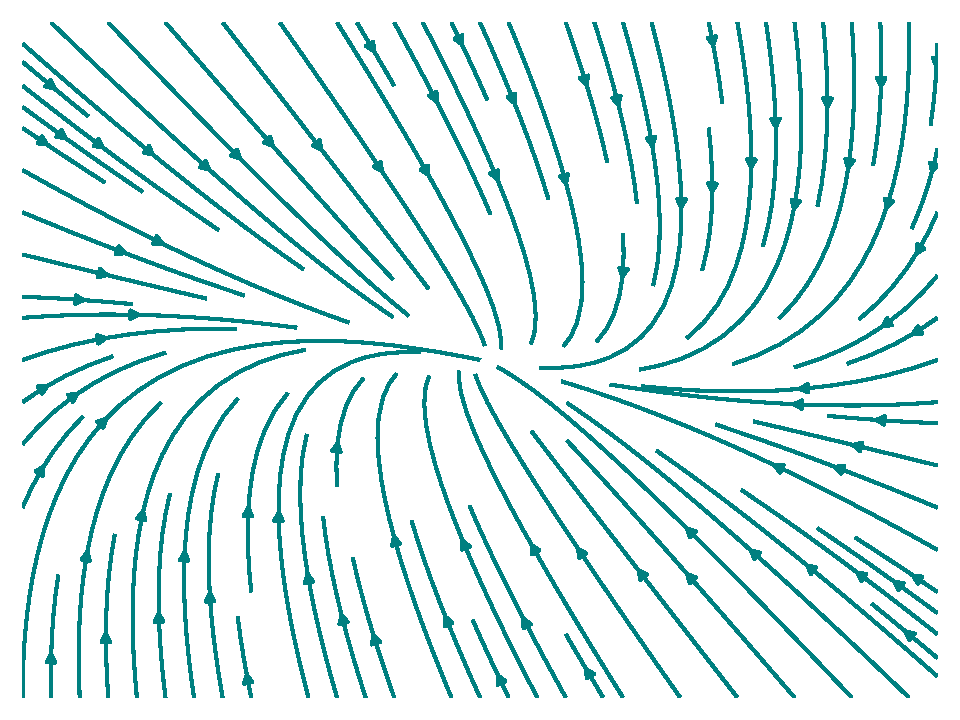
\includegraphics[width=7cm]{nó estável.pdf} 
	\end{figure}
	%
	\lstinputlisting[language=Python, caption=Código Python para ilustrar o retrato de fase]{phase portrait.py}
	
	\noindent
	\textbf{\sffamily Exercício 2 --- solução.} \\
	O ponto de equilíbrio é novamente o $(0,0)$. 
	Na verdade, este é o equilíbrio em todos os exercícios.
	Calculando os autovalores, temos
	%
	\begin{align*}
		\det(\lambda\I - A) = 0 \implies
		\det
		\begin{pmatrix}
			\lambda+2 & 4 \\
			4 & \lambda+2
		\end{pmatrix}
		&= 0 \\
		\iff
		(\lambda+2)(\lambda+2) - 16 &= 0 
		\implies 
		\lambda = -2 \pm 4,
	\end{align*}
	%
	isto é, autovalores de sinais distintos. 
	Isso mostra que a origem é ponto de sela do retrato, e a próxima tarefa é encontrar as direções (autovetores) de divergência ($v_d$) e convergência ($v_c$) por esse ponto. 
	Daí,
	%
	\begin{align*}
		Av_d = 2v_d \iff v_d = \alpha\binom{1}{-1} ,
		\quad
		Av_c = 2v_c \iff v_c = \alpha\binom{1}{1} . 
	\end{align*}
	%
	O retrato fica
	%
	\begin{figure}[H]\centering
		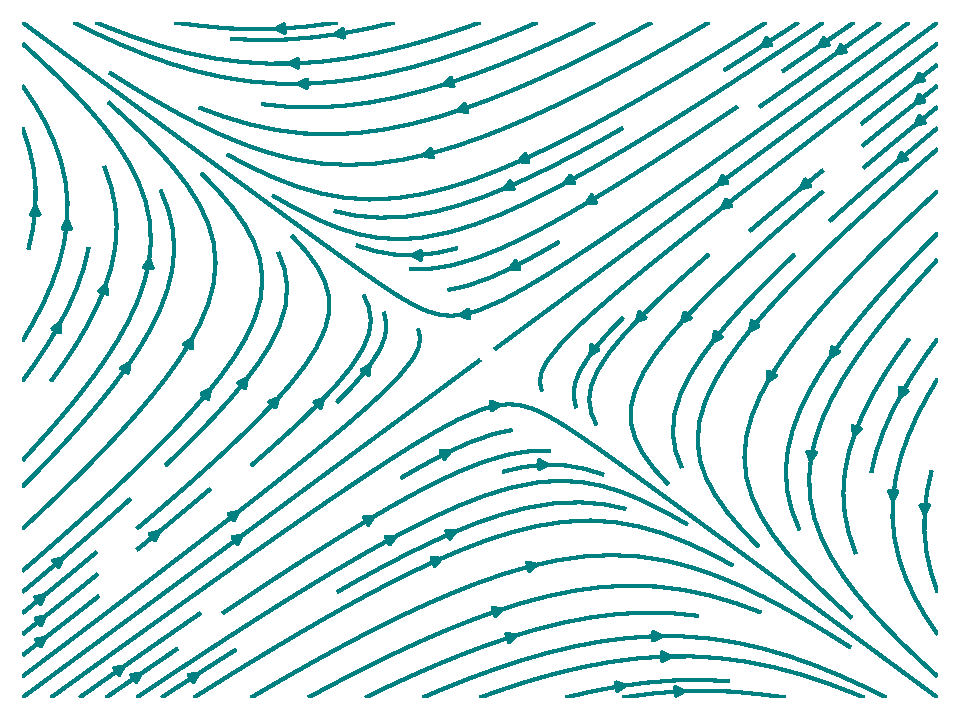
\includegraphics[width=7cm]{sela.pdf} 
	\end{figure}
	%
	
	\noindent
	\textbf{\sffamily Exercício 3 --- solução.} \\
	Ao contrário dos exercícios anteriores, estas EDs não são lineares, e o que buscaremos achar é apenas uma tentativa de aproximação local na origem. 
	Linearizando nessa região, 
	%
	\begin{align*}
		\dot{X} \approx 
		\begin{pmatrix}
			0 & 1 \\
			-1 - 2\bar{x_1}\bar{x_2} & 1-\bar{x_1}^2
		\end{pmatrix}
		X
		=
		\begin{pmatrix}
			 0 & 1 \\
			-1 & 1
		\end{pmatrix}
		X,
	\end{align*}
	%
	e segue daí que¨
	%
	\begin{align*}
		\det(\lambda\I - A) = 0 \implies 
		\det
		\begin{pmatrix}
			\lambda & -1 \\
			1 & \lambda-1
		\end{pmatrix}
		&= 0 \\
		\iff
		\lambda(\lambda-1) + 1 &= 0
		\implies 
		\lambda = \frac{1}{2} \pm i\frac{\sqrt{3}}{2}.
	\end{align*}
	%
	Como os autovalores têm parte real positiva e parte imaginária não nula, trata-se de um foco instável. 
	O interessante da equação de Van der Pol, entretanto, é que para $x_1$ suficientemente grade, o sistema deixa de divergir e ``entra em loop"; 
	em outras palavras, a instabilidade do foco pode levar o sistema a um comportamento oscilatório. 
	Vide o retrato a seguir.
	%
	\begin{figure}[H]\centering
		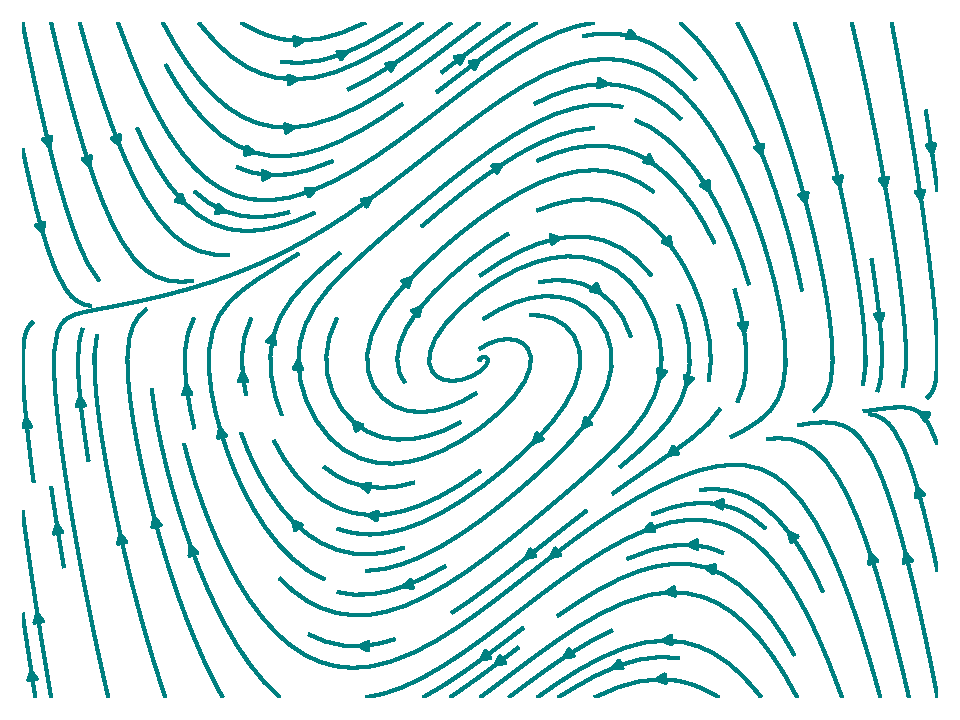
\includegraphics[width=7cm]{van der pol.pdf}
	\end{figure}
	%
	
	\noindent
	\textbf{\sffamily Exercício 4 --- solução.} \\
	Em outras palavras, queremos verificar que 
	$H(x)\geq 0$, 
	$H(\bar{x})=0$ e 
	$\dot{H}(x(t)) \leq 0$ para a EDO massa-mola 
	%
	\[
		m\ddot{x} + kx = 0.
	\]
	%
	As primeiras duas igualdades são triviais; quanto à última, temos 
	%
	\begin{align*}
		\dot{H} &= \frac{d}{dt} \left(
		               \frac{m\dot{x}^2}{2} + 
		               \frac{kx^2}{2}
		           \right) \\
		        &= \frac{m}{2} (2\dot{x}\ddot{x}) +
		           \frac{k}{2} (2x\dot{x}) \\
		        &= \dot{x}
		           \underbrace{(m\ddot{x} + kx)}_{=0} 
		        \equiv 0.
	\end{align*} 
	%
	Logo o sistema é de fato estável e $H$ é uma função de Lyapunov. \\
	%
	
	\noindent
	\textbf{\sffamily Exercício 5 --- solução.} \\
	Desta vez, tratamos do sistema 
	%
	\[
		m\ddot{x} + \alpha \dot{x}|\dot{x}| + kx = 0,
	\]
	% 
	onde $\alpha$ é o coeficiente de atrito viscoso.
	Prosseguindo de maneira idêntica à questão anterior, encontramos
	%
	\begin{align*}
		\dot{H} &= \dot{x}(m\ddot{x} + kx) \\
		        &= \dot{x}(-\alpha\dot{x}|\dot{x}| - kx + kx) \\
		        &= -\alpha\dot{x}^2|\dot{x}| 
		        < 0 \quad\forall x\neq 0.
	\end{align*}
	%
	Logo o sistema é assintoticamente estável (desigualdade estrita).
	
	
	